\documentclass[11pt,a4paper]{article}
\usepackage[utf8]{inputenc}
\usepackage[T1]{fontenc}
\usepackage[english]{babel}
\usepackage{lmodern}
\usepackage{amsmath}
\usepackage{amsfonts}
\usepackage{amssymb}
\usepackage{amsthm}
\usepackage{verbatim}

\usepackage{qtree}

\usepackage{ifthen}
\usepackage[framemethod=tikz]{mdframed}
\usepackage{tikzpagenodes}
\usetikzlibrary{calc, arrows}

\newcounter{Exo}[section]

% greyarrow has much better handling of page breaks, see the link on stackoverflow for more info
\def\SolStyle{greyarrow}
\ifthenelse{\isundefined{\SolStyle}}{\def\SolStyle{greyarrow}}{}
\ifthenelse{\equal{\SolStyle}{greyarrow}}
{
  %http://tex.stackexchange.com/questions/50877/excursus-environment-using-mdframed-issue-with-page-breaks
\tikzset{
   excursus arrow/.style={%
    line width=2pt,
    draw=gray!40,
    rounded corners=2ex,
   },
   excursus head/.style={
    fill=white,
    font=\bfseries\sffamily,
    text=gray!80,
    anchor=base west,
   },
}

\mdfdefinestyle{mysquare}{%
  singleextra={%
   \path let \p1=(P), \p2=(O) in (\x2,\y1) coordinate (Q);%
   \path let \p1=(Q), \p2=(O) in (\x1,{(\y1-\y2)/2}) coordinate (M);%
   \path [excursus arrow, round cap-to]%
   ($(O)+(5em,0ex)$) -| (M) |- %
   ($(Q)+(12em,0ex)$) .. controls +(0:16em) and +(185:6em) .. %
   ++(23em,2ex);%
   \node [excursus head] at ($(Q)+(2.5em,-0.75pt)$) {Solution to Exercise~\theExo};},
  firstextra={%
   \path let \p1=(P), \p2=(O) in (\x2,\y1) coordinate (Q);
   \path [excursus arrow,-to]
   (O) |- %
   ($(Q)+(12em,0ex)$) .. controls +(0:16em) and +(185:6em) .. %
    ++(23em,2ex);
   \node [excursus head] at ($(Q)+(2.5em,-2pt)$) {Solution to Exercise~\theExo};
  },
  secondextra={%
   \path let \p1=(P), \p2=(O) in (\x2,\y1) coordinate (Q);
   \path [excursus arrow,round cap-]
   ($(O)+(5em,0ex)$) -| (Q);
  },
  middleextra={%
   \path let \p1=(P), \p2=(O) in (\x2,\y1) coordinate (Q);
   \path [excursus arrow](O) -- (Q);
 },
 middlelinewidth=2.5em,middlelinecolor=white,
 hidealllines=true,topline=true,
 innertopmargin=0.5ex,
 innerbottommargin=2.5ex,
 innerrightmargin=2pt,
 innerleftmargin=2ex,
 skipabove=0.87\baselineskip,
 skipbelow=0.62\baselineskip,
}

}
{
  \input{boxes.tex}
}

\newenvironment{solution}{\stepcounter{Exo}\begin{mysolution}}{\end{mysolution}}
\newmdenv[style=mysquare]{mysolution}

\usepackage{url}
\newcommand{\newape}[1]
{\section{Practical Session \thesection ( #1 )}}
\newcommand{\nosolution}
{\begin{mysolution}\stepcounter{Exo}
The exercise~\theExo{} does not yet have a solution.
You are encouraged to submit one to the following address
\begin{center}
  \url{https://github.com/Gp2mv3/ELEC2795}
\end{center}
or by mail to \url{nicolascognaux@gmail.com}.\end{mysolution}}

\newcommand{\copyapeexo}[2]
{\begin{mysolution}See APE#1, exercise~#2.\end{mysolution}}


\newcommand{\xor}{\oplus}

\newcommand{\A}{\mathcal{A}}
\newcommand{\D}{\mathcal{D}}
\newcommand{\C}{\mathcal{C}}
\newcommand{\K}{\mathcal{K}}
\newcommand{\M}{\mathcal{M}}
\newcommand{\G}{\mathcal{G}}
\DeclareMathOperator{\Gen}{\mathsf{Gen}}
\DeclareMathOperator{\Enc}{\mathsf{Enc}}
\DeclareMathOperator{\Dec}{\mathsf{Dec}}
\DeclareMathOperator{\Mac}{\mathsf{Mac}}
\DeclareMathOperator{\Vrfy}{\mathsf{Vrfy}}
\DeclareMathOperator{\Com}{\mathsf{Com}}
\DeclareMathOperator{\Open}{\mathsf{Open}}
\DeclareMathOperator{\Sign}{\mathsf{Sign}}
\DeclareMathOperator{\Sig}{\mathsf{Sig}}

\DeclareMathOperator{\PrivK}{PrivK}
\DeclareMathOperator{\MacForge}{MacForge}
\DeclareMathOperator{\Sigforge}{Sig-forge}
\DeclareMathOperator{\Invert}{Invert}
\DeclareMathOperator{\DDH}{DDH}
\DeclareMathOperator{\DLog}{DLog}
\newcommand{\PrivKeav}{\PrivK^{\text{eav}}}
\newcommand{\PrivKmultcpa}{\PrivK^{\text{multcpa}}}
\newcommand{\Sigforgeone}{\Sigforge^{\text{1--time}}}

\DeclareMathOperator{\Ima}{\mathsf{Im}}

\title{Solutions of the exercises of ELEC2795}
\author{Nicolas Cognaux}

\begin{document}

\maketitle
\tableofcontents

\newape{Plane wave}
For this one, we have the solution, see {\bf LELEC2795 exercice solution plane waves.pdf} on iCampus.
\newape{Transmission Lines}
For this one, we have the solution, see {\bf LELEC2795 exercices and solutions transmission lines.pdf} on iCampus.
\newape{Antennas and radiating Systems}

\begin{solution}
	There are two paths. The direct one and the reflected. The direct distance is $D = \sqrt{d^2 + (h_1 - h_2)^2} \approx d$. Using the information given in the exercise ($E(d) = \frac{k\sqrt{P}}{d}$), we have a first component of the received field equal to $E(d) = \frac{k\sqrt{P}}{D}$.

	
	The second distance is longer: $D_{refl}(a) = \sqrt{h_1^2 + a^2} + \sqrt{h_2^2 + (d - a)^2}$ with $a \in [0:d]$. 	
	The reflection parameters given are $(\rho, \alpha)$ where I think, $\rho$ is the reflection ratio where $\alpha$ is the angle between the incident and the reflection field. So we have $a = h_1 \tan{\alpha/2}$ and $d - a = h_2 \tan{\alpha/2}$. 
	The second electric field is then: $E_{refl} = \frac{k\sqrt{P}}{(h_1 + h_2)(1 + \tan{\alpha/2})}\rho$.
	
	
	Finally, the received electric field is the sum:
	$$E_{tot} = k\sqrt{P} (\frac{1}{(h_1 + h_2)(1 + \tan{\alpha/2})}\rho + \frac{1}{\sqrt{d^2 + (h_1 - h_2)^2}}$$

	
	The simplification $\rho = 1, \alpha = \pi$ conduct to a big simplification (the ground can be ignored) so that it only remains the direct path: $E_{tot} = \frac{k\sqrt{P}}{d}$.
\end{solution}

\begin{solution}
	\begin{enumerate}
		\item The power density decreases in $\frac{1}{4\pi d^2}$ with $d \approx 141.4m$ via Pythagore:
			  $$ S = \frac{1}{4\pi 141.4^2} = 3.98\expten{-6}_W/m^2 $$
		\item $E_0 = E \cdot \hat{a_z} \exp{-j\vec{k} \cdot \vec{r}}$ where $\vec{r}$ is directed toward the center of the plate.
		\item It's the same expression with $\vec{r} = \frac{(a_x, a_y, 0)}{\sqrt{2}}$ and $\vec{k} = k \hat{a}$. Then we have 
			  $$E_{inc} = E \cdot \hat{a_z} \exp{-j k (a_x + a_y)/\sqrt{2}}$$ 

			  \notsure
			  
		\item We can define the origin at the reflection point, so that we have an incident wave coming with angle $\alpha = \pi/4$. The reflected magnetic field is given by the expression of $H_r$ of the second slide of page 12 from the propagation fundamentals course.
			  \notsure I don't know how to compute the induced current...
		\item Without the expression of the current I cannot have an expression here... \notsure
	\end{enumerate}
\end{solution}

\begin{solution}
	$d = 1km$, $f = \expten{3} MHz$, $P = 1W = 1000 mW$.
	If we use the formula given by the second slide of page 6 of the Antenna course.
	$$\epsilon = 32.5 + 20 \log \expten{3} + 20 \log 1 - 2.15 - 10\log (0.7\frac{\pi 1^2}{4}\frac{4\pi \expten{9}}{3 \expten{8}}) = 76.7dB$$
	With $G_R = 2.15 dB$ for a Dipole (first slide pg 8).  
	
	So the final answer is:
	$$P = 10 \log \expten{3} - \epsilon = -46.7dB$$
\end{solution}

\begin{solution}
	

\end{solution}


\nosolution
\nosolution
\nosolution
\newape{Cellular Systems}

\begin{solution}
	\begin{enumerate}
	\item
		We can assume that the signal is polarized $//$ to the reflection plane so that the polarization is not affected.
		
		
		The received signal is the sum of two: $E = E_d + E_r$. The direct one will only be affected by the path loss:  $E_d = E\frac{e^{-j\vec{\beta} \vec{r}}}{r}$ while the second will also be affected by the reflection, in addition to the longer path:
		$E_r = E\frac{e^{-j\vec{\beta} \vec{r'}}}{r'}$ with $r' \approx r$.
		Then the normalized sum is simply $E_n = 1 + \frac{r'}{r}e^{-j\beta(r' - r)} =  1 + \alpha e^{-j\beta\Delta r}$. We can then draw the plot from $0$ to $2\pi$.
		
		%Figure \ref{fig:tp4ex1} shown this graph.
		%\begin{figure}[h]
		%	\centering
		%	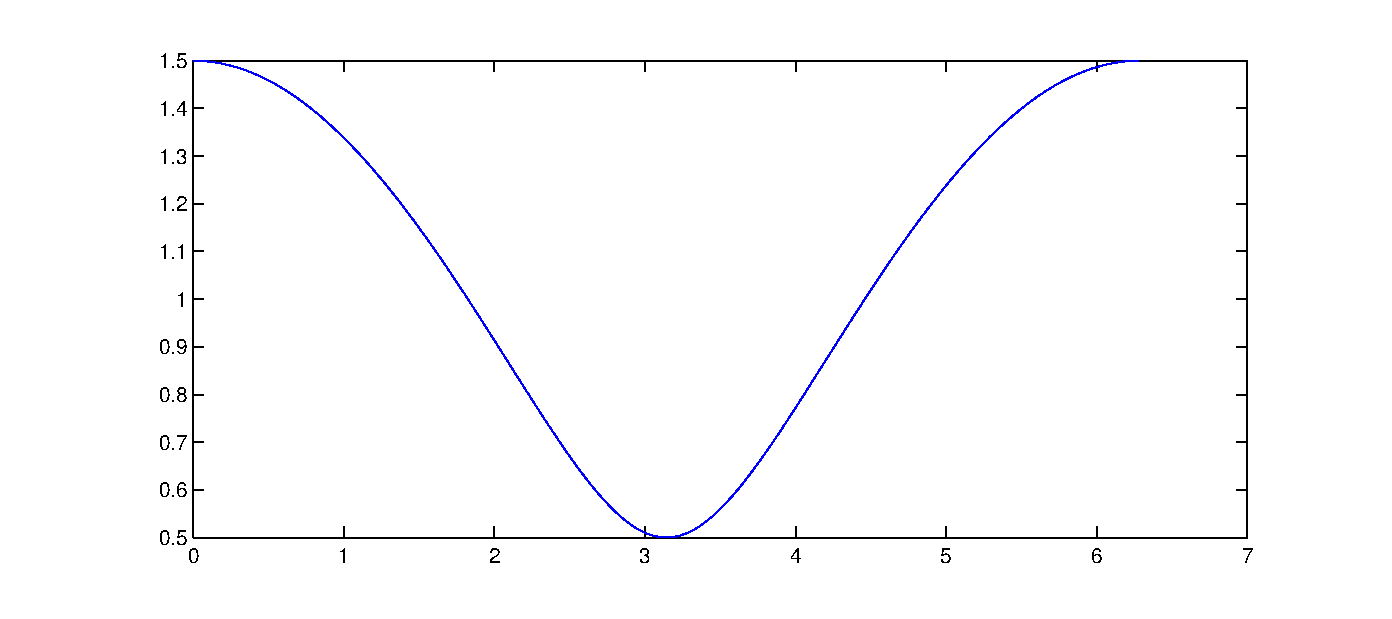
\includegraphics[width=0.4\linewidth]{tp4ex1.eps}
		%	\caption{Normalized received signal}
		%	\label{fig:tp4ex1}
		%\end{figure}	
		
	\item Now that there is a movement, the phase shift is also due to the speed (Doppler shift). So we will use the equation:
	$$ \frac{2\pi}{c}f_c \sin \theta v \Delta t = \frac{2\pi}{\lambda} \sin \theta v \Delta t$$
	Here $\theta = 40^\circ \rightarrow \sin \theta = \frac{\sqrt{2}}{2}$
	
	So $E = E_d + E_d e^{j\frac{2\pi}{\lambda}\frac{\sqrt{2}}{2}v t}$, then, if we compute $E(t_2) - E(t_1) = E e^{j \frac{2\pi}{\lambda} \frac{\sqrt{2}}{2} v t_2} (1 - e^{v (t_1 - t_2)}) = E e^{j \frac{2\pi}{\lambda} \frac{\sqrt{2}}{2}v t_2}(1 - e^{\Delta d})$.
	Then, after normalization, we obtain:
	$$E_n = (1 - e^{\Delta d})$$
	
	\end{enumerate} 
\end{solution}

\begin{solution}
	\begin{enumerate}
		\item We know that the path loss is defined as $P = \frac{4\pi r}{\lambda}^2$ with d the distance, then, if we want a maximal attenuation of $140dB = 1\expten{-14} W$, we can simply replace the variables and retrieve:
		$d_{900} = 265258m$, $d_{1800} = 132629m$
		
		\item If we use the lognormal distribution (corresponding to the shadowing distribution), we can recover $P(X \leq x) = 0.95 = 0.5 erfc(\frac{x - \mu}{\sigma \sqrt{2}}) \rightarrow X = 1.25$. Then we have to "de-normalize" it via: $X = \frac{x - \mu}{\sqrt{2} \sigma}$ so $\mu = x - X\sqrt{2}\sigma = 140 - 1.25\sqrt{2}6 = 129.4dB$.
		So the new distances are: $d_{new~900} = 247553m$, $d_{new~1800} = 123776m$.
		
		At the exercise session, we found something realy smaller than before. I think the assistant forgot to convert $\mu$ fro dB to Watts. \notsure
	\end{enumerate}
\end{solution}

\nosolution

\newape{Digital Transmission}

\begin{solution}
	$$\int_0^\infty P_e P_\gamma d\gamma = \frac{1}{2} \int_0^\infty erfc(\sqrt{\gamma}) \frac{e^{\frac{-\gamma}{\beta}}}{\beta} d\gamma$$
	We use the composed integration with $f = \frac{1}{2}erfc{\sqrt{\gamma}} \rightarrow f' = \frac{-1}{\sqrt{\pi}}\frac{e^{-\gamma}}{\sqrt{\gamma}}$ and $g' = \frac{e^{\frac{-\gamma}{\beta}}}{\beta} \rightarrow g = e^{\frac{-\gamma}{\beta}}$.
	Then we replace the variable $d\gamma \rightarrow d\gamma \sqrt{1 + \frac{1}{\beta}}$. 
	
	Finally, we obtain the expression of the average BER:
	$$\overline{BER} = \frac{1}{2}(1 - \sqrt{\frac{1}{1 + \beta}})$$
	Where $\beta = SNR$, that corresponds to the expression 28 of slide 10 about OFDM.
\end{solution}

\begin{solution}
	$s = P d$ where d is the data and $P$ is the precoding matrix, then we have $y = Gs + n = GPd + n$, where $G$ is the FIR representation of the channel and $n$ is the noise (AWGN).
	We know that the channel has a frequency response $\Omega$. So we can say that $G = W^H \Omega W$ where $W$ is the FFT matrix (as defined in the exercise).
	We have $y = W^H \Omega W P d + n = W^H \Omega W d + n$. As we are in single carrier, $P = I_{n \times n}$.
	
	The zero-forcing equalizer will apply the inverse of the channel frequency response (estimated before), so we have:
	$$\hat{d} = W^H \Omega^{-1} W y = d + W^H \Omega^{-1}W n$$
	
	The SNR can then be expressed with that previous expression:
	$$SNR = \frac{|Signal|^2}{|Noise|^2} = \frac{|d|^2}{|W^H \Omega^{-1}W n|^2}$$
	This can then be expressed with a sum because we know that the matrix of noise will be circulant: 
	$$W^H \Omega^{-1}W = \frac{1}{\sqrt{K}}\sum^{K-1}_{k = 0} \sum^{K-1}_{k' = 0} e^{-jkk'/K} \frac{1}{\omega_k} \sum^{K-1}_{k' = 0} e^{jkk'/K} = \frac{1}{K} \sum^{K-1}_{k = 0} \frac{1}{\omega_k}$$
	
	$$
	SNR = \frac{1}{| \frac{1}{K} \sum^{K-1}_{k = 0} \frac{1}{\omega_k}n|^2} = \frac{1}{\frac{1}{K} \sum^{K-1}_{k = 0} \frac{|n|^2}{h_k}}
	$$
	
	We also know that $|n|^2 = \sigma_n$	, which simplify the expression to :
	$$SNR = \frac{1}{\frac{1}{K} \sum^{K-1}_{k = 0} \frac{\sigma_n}{h_k}}$$
\end{solution}
\newape{DSL Systems}

\nosolution
\nosolution
\newape{Positionning}

\nosolution


\end{document}
